\documentclass{beamer}
\usetheme{Metropolis}
\setbeamercovered{transparent}

%Metropolis, CambridgeUS

\usepackage{hyperref}
\usepackage{amsmath}
\usepackage{xcolor}
\usepackage{tabularx} % Para tablas que se ajustan al ancho
\usepackage{rotating} % Para tablas giradas

\title[Aprendizaje automático orientado a la clasificación de cáncer de piel]{Aprendizaje automático orientado a la clasificación de cáncer de piel: un enfoque basado en EfficientNetB1}
\author{
    Deborah Famadas Rodríguez\\
    \small{Tutores:}\\
    Dr. Reinaldo Rodríguez Ramos$^{*}$\\
    Dr. Yudivian Almeida Cruz
}
\institute{
    Universidad de la Habana (UH) \\
    $^{*}$Universidade Federal Fluminense (UFF), Rio de Janeiro, Brasil\\
    \vspace{0.25cm}
    \href{https://github.com/deborahfam/Thesis}{github.com/deborahfam/Thesis}
}
\date{\today}
\logo{
\includegraphics[height=1cm]{Graphics/uhlogo}}

\begin{document}

\frame{\titlepage}

\begin{frame}
  \frametitle{Cáncer de piel}

  \begin{figure}[H]
    \begin{center}
      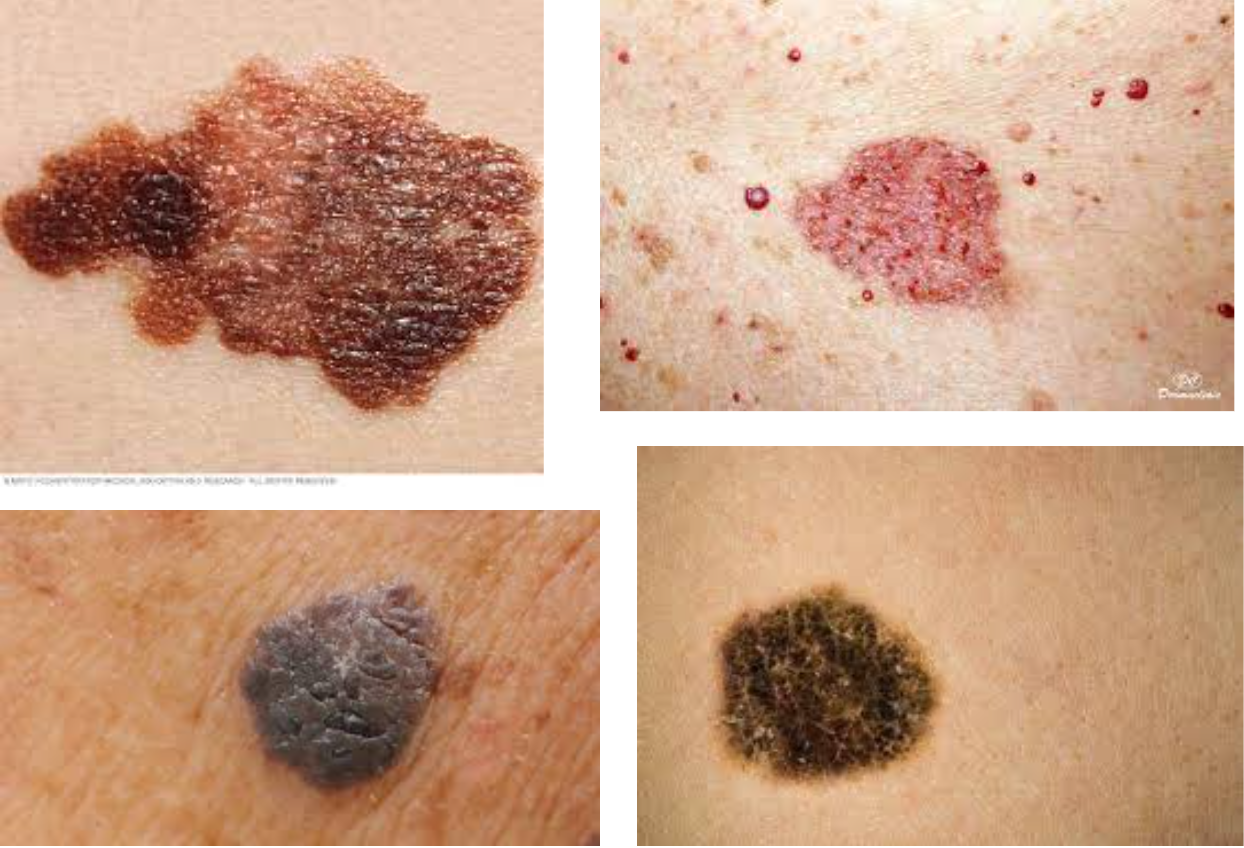
\includegraphics[width=1\textwidth]{./Graphics/skin_cancer.drawio.png}
      \label{fig:skin-cancer}
    \end{center}
  \end{figure}
\end{frame}


\begin{frame}
  \frametitle{Aprendizaje automático}

  \begin{figure}[H]
    \begin{center}
      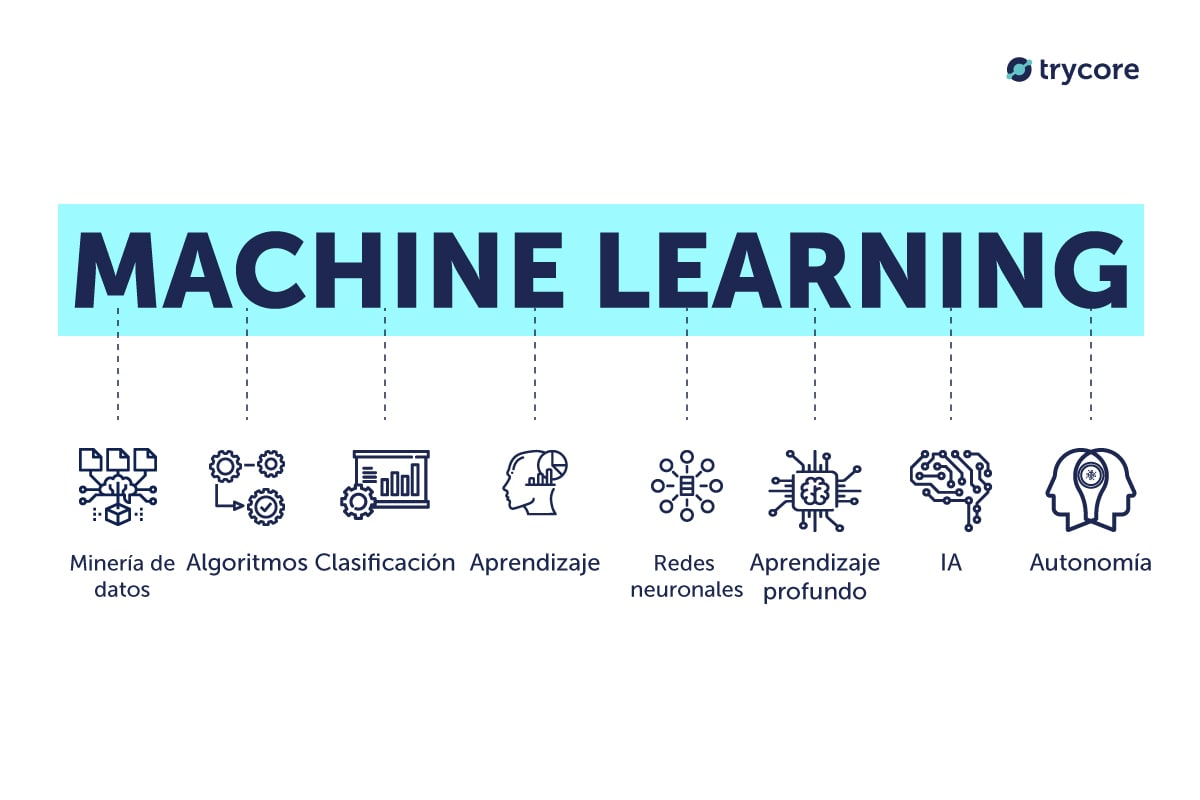
\includegraphics[width=1\textwidth]{./Graphics/ml.jpg}
      \label{fig:ml}
    \end{center}
  \end{figure}
\end{frame}


\begin{frame}
  \frametitle{Objetivos}

  \begin{block}{Propósito central}<1->
    \vspace{2mm}
    Desarrollar un modelo de \textit{deep learning} para el diagnóstico de cáncer de piel a través de la clasificación de imágenes dermatológicas.
  \end{block}

    \begin{block}{Propósitos específicos}<2->
      \small
      \begin{enumerate}
        \item<3-> Estudio del estado del arte en diagnóstico de imágenes dermatológicas.
        \item<4-> Desarrollo de un modelo de \textit{deep learning} para clasificación.
        \item<5-> Optimización de la distribución de datos.
        \item<6-> Mejoras y ajuste de hiperparámetros.
        \item<7-> Implementación de técnicas de validación.
      \end{enumerate}
    \end{block}
\end{frame}


\begin{frame}
  \frametitle{Redes Neuronales Convolucionales en Medicina}

  \begin{block}{¿Qué son las CNNs?}
  \end{block}

  \pause
  \note[cnn]{Las redes neuronales convolucionales (CNN) son un subconjunto de aprendizaje automático y están en el centro de los algoritmos de aprendizaje profundo. Estan especialmente diseñadas para el procesamiento de imágenes, las CNN son capaces de capturar patrones espaciales y temporales en los datos.}

  \begin{block}{Componentes de la arquitectura de las CNNs}
    % \small
    % \begin{itemize}
    %   \item<3-> Capa convolucional (\textit{Convolutional layer}).
    %   \item<4-> Capa de agrupación (\textit{Pooling layer}).
    %   \item<5-> Capa de función de activación (\textit{ReLu}).
    %   \item<6-> Capa completamente conectada (\textit{Full connected layer}).
    % \end{itemize}

    \begin{figure}[H]
      \begin{center}
        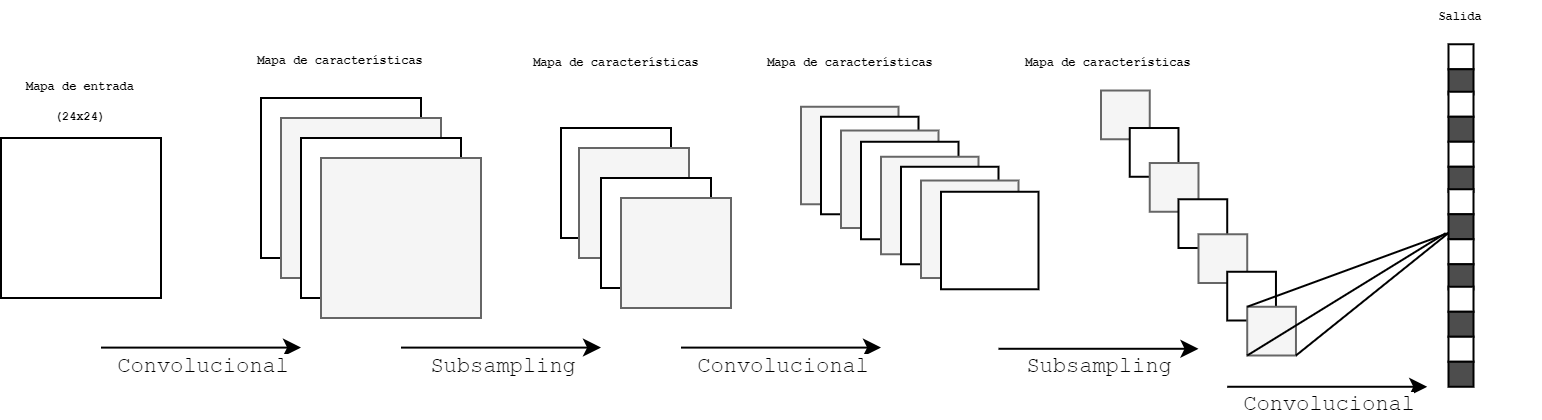
\includegraphics[width=1\textwidth]{./Graphics/cnn.drawio.png}
        \caption{Estructura de una red neuronal convolucional.}
        \label{fig:cnn-convol}
      \end{center}
    \end{figure}
    
  \end{block}
\end{frame}


\begin{frame}
  \frametitle{Objetivos}

    \begin{block}{Propósitos específicos}
      \small
      \begin{enumerate}
        \item<0-> Estudio del estado del arte en diagnóstico de imágenes dermatológicas.
        \item<0> Desarrollo de un modelo de \textit{deep learning} para clasificación.
        \item<0> Optimización de la distribución de datos.
        \item<0> Mejoras y ajuste de hiperparámetros.
        \item<0> Implementación de técnicas de validación.
      \end{enumerate}
    \end{block}
\end{frame}

\begin{frame}
  \frametitle{Red neuronales pre-entrenadas}

  \begin{enumerate}
    \small
    \item Generales o profundas
    \item De varias capas (\textit{multilayers}).
    \item Completamente conectadas (\textit{fully connected}).
  \end{enumerate}

  \note[options]{Aprovechar el conocimiento de una tarea para resolver otra, Acelera el aprendizaje, Mejora la generalización y reconocimiento de patrones en imágenes dermatoscópicas.}

  \begin{block}{Transferencia de aprendizaje (\textit{transfer learning})}
    \begin{figure}[H]
      \begin{center}
        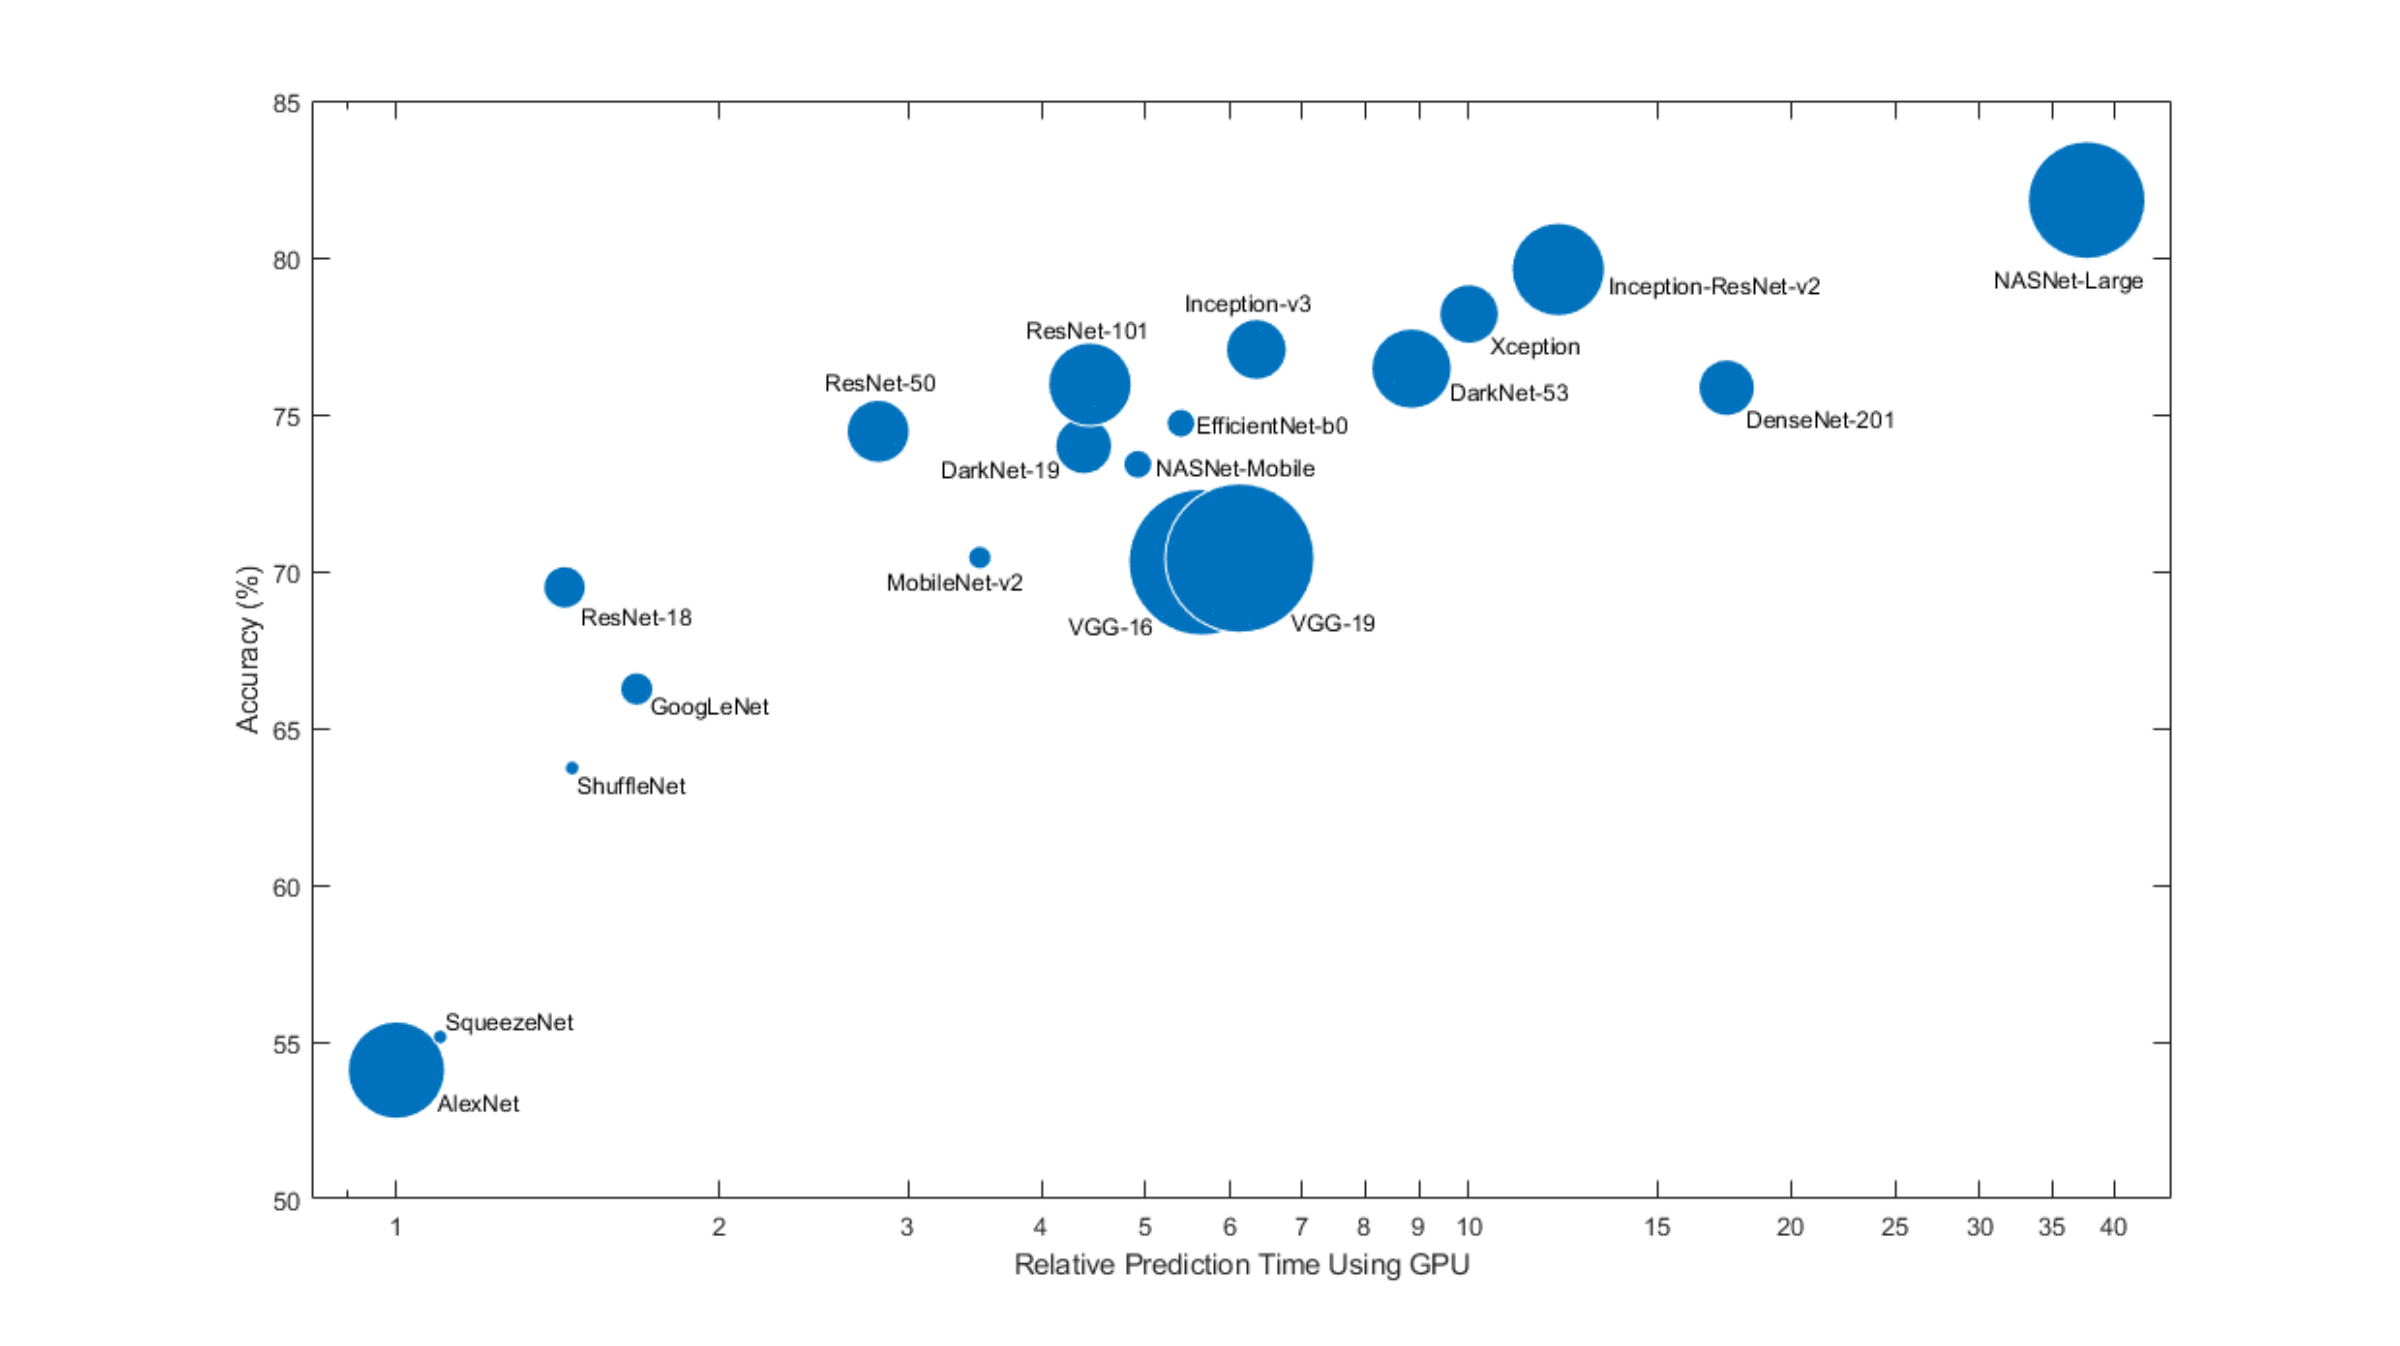
\includegraphics[width=0.75\textwidth]{./Graphics/pre-trained-cnn.drawio.png}
        \caption{Algoritmos de transferencia de aprendizaje.}
        \label{fig:pre-trained}
      \end{center}
    \end{figure}
  \end{block}
\end{frame}


\begin{frame}
  \frametitle{Objetivos}

    \begin{block}{Propósitos específicos}
      \small
      \begin{enumerate}
        \item<0> Estudio del estado del arte en diagnóstico de imágenes dermatológicas.
        \item<0-> Desarrollo de un modelo de \textit{deep learning} para clasificación.
        \item<0-> Mejoras y ajuste de hiperparámetros.
        \item<0> Optimización de la distribución de datos.
        \item<0> Implementación de técnicas de validación.
      \end{enumerate}
    \end{block}
\end{frame}

\begin{frame}
  \frametitle{Propuesta de Solución}
  \begin{itemize}
    \item <1-> Una red neuronal convolucional propia que utiliza como entrada los pesos obtenidos de una red neuronal convolucional pre-entrenada, EfficientNetB1.
    \item <2-> Algoritmo propio para ajuste de precisión.
  \end{itemize}
\end{frame}

\begin{frame}
  \frametitle{EfficientNet}
  \begin{figure}[H]
    \begin{center}
      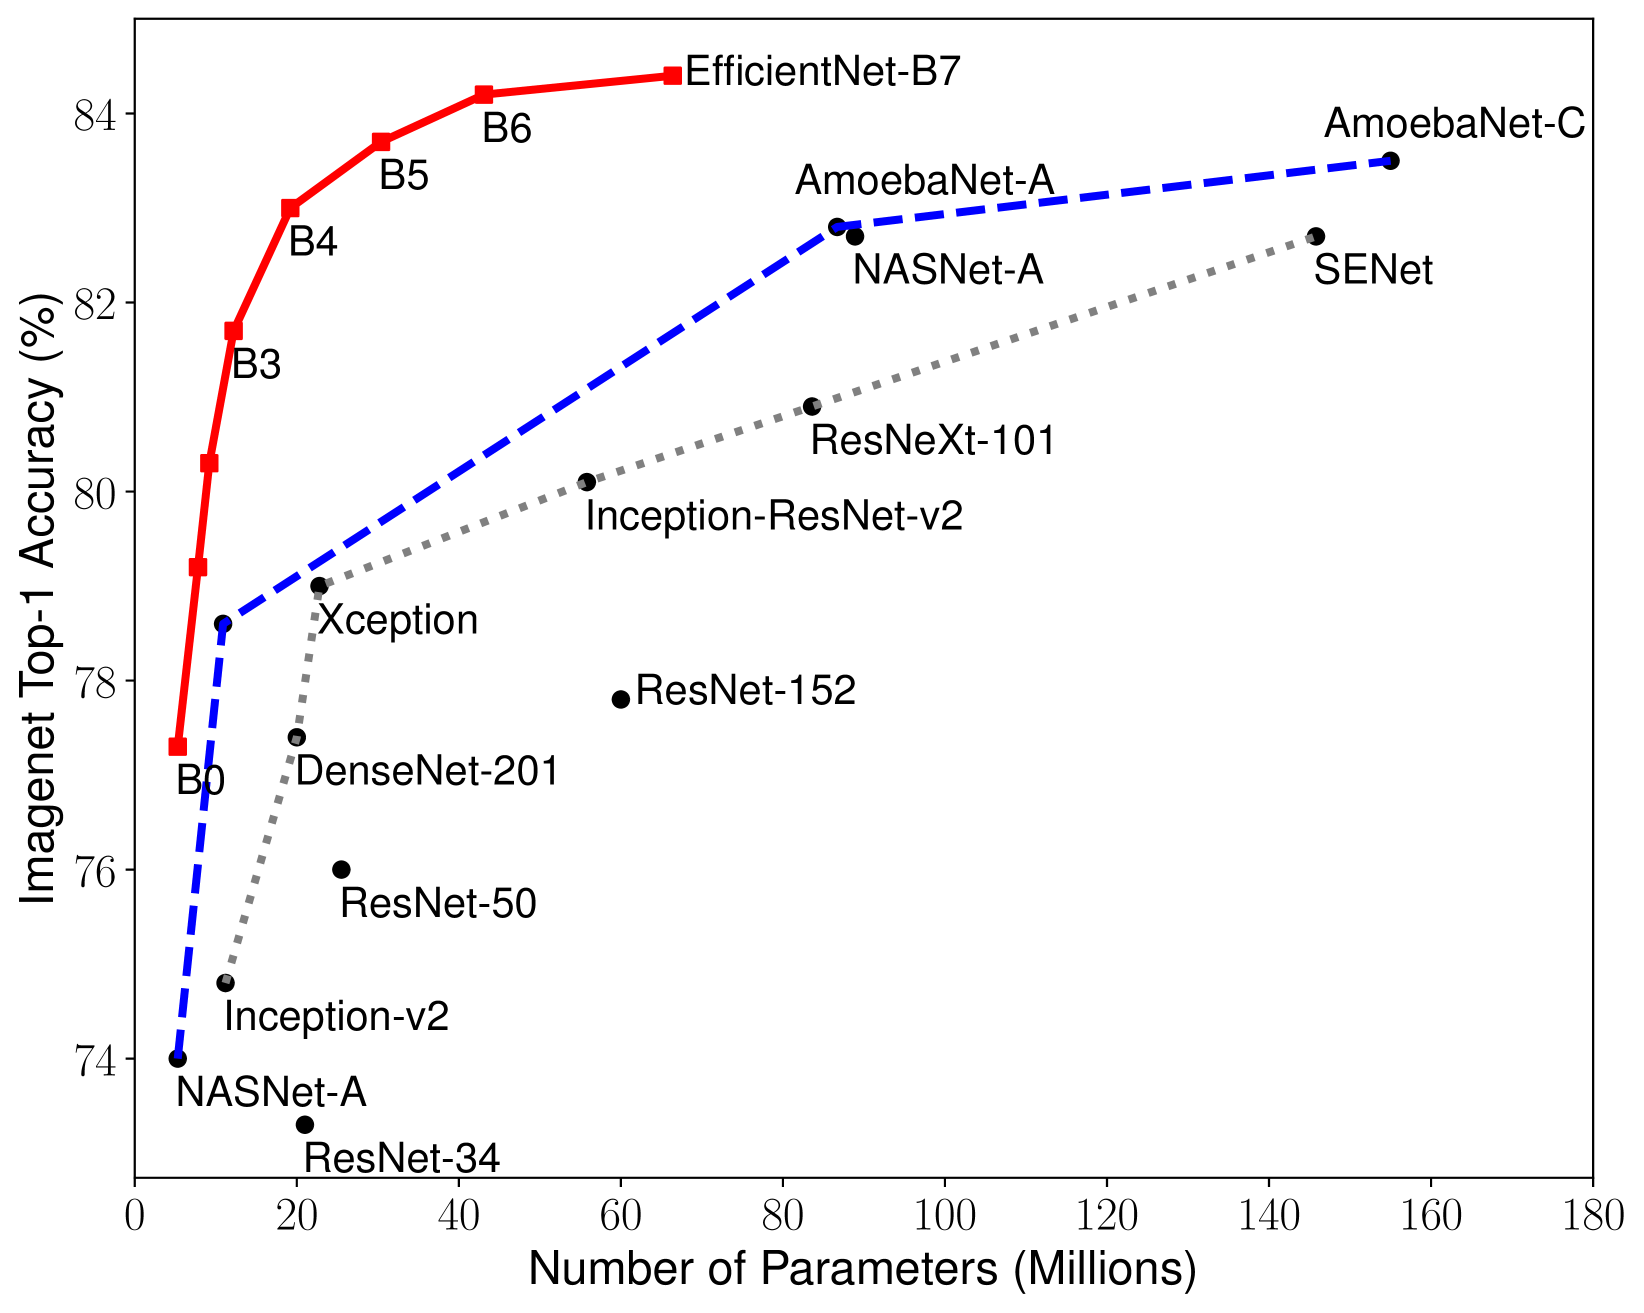
\includegraphics[width=0.8\textwidth]{./Graphics/efficientnet_performance.png}
      \caption{Desempeño de los modelos de EfficientNet.}
      \label{fig:pre-trained-cnn}
    \end{center}
  \end{figure}
\end{frame}

\begin{frame}
  \frametitle{Propuesta de Solución}
  \begin{itemize}
    \item <0-> Una red neuronal convolucional propia que utiliza como entrada los pesos obtenidos de una red neuronal convolucional pre-entrenada, EfficientNetB1.
    \item <0> Algoritmo propio para ajuste de precisión.
  \end{itemize}
\end{frame}

\begin{frame}
  \frametitle{Modelo y capas adicionales}
  \begin{itemize}
    \item Capa de normalización.
    \item Capa densa y regularización.
    \item Capa de \textit{dropout}.
    \item Capa de salida con activación \textit{softmax}.
  \end{itemize}

  \begin{figure}[H]
    \begin{center}
    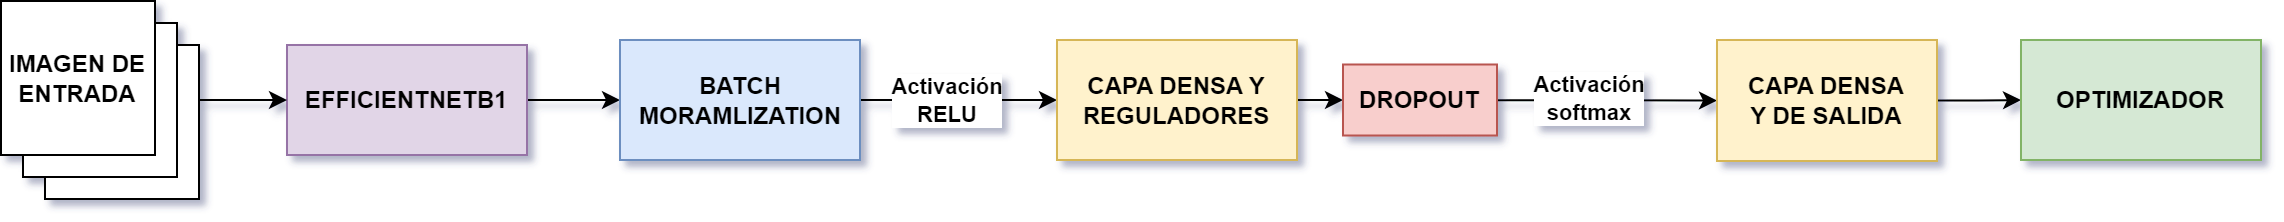
\includegraphics[width=1\textwidth]{./Graphics/diagrama_modelo.drawio.png}
    \caption{Diagrama del modelo propuesto.}
    \label{fig:model_permormance}
    \end{center}
  \end{figure}


 \textbf{Tasa de Aprendizaje Inicial:} $0.001$, \\ \textbf{Regularización:} L2 con $\lambda = 0.016$ y L1 con $\lambda = 0.006$, \\ \textbf{Dropout:} 45\%, \\ \textbf{Dimensiones de la Imagen:} $224 \times 224 \times 3$, \\ \textbf{Optimizador:} Adamax
\end{frame}

\begin{frame}
  \frametitle{Propuesta de Solución}
  \begin{itemize}
    \item <0> Una red neuronal convolucional propia que utiliza como entrada los pesos obtenidos de una red neuronal convolucional pre-entrenada, EfficientNetB1.
    \item <0-> Algoritmo propio para ajuste de precisión.
  \end{itemize}
\end{frame}

\begin{frame}
  \frametitle{Ajuste de tasa de aprendizaje}
  \begin{figure}[H]
    \begin{center}
    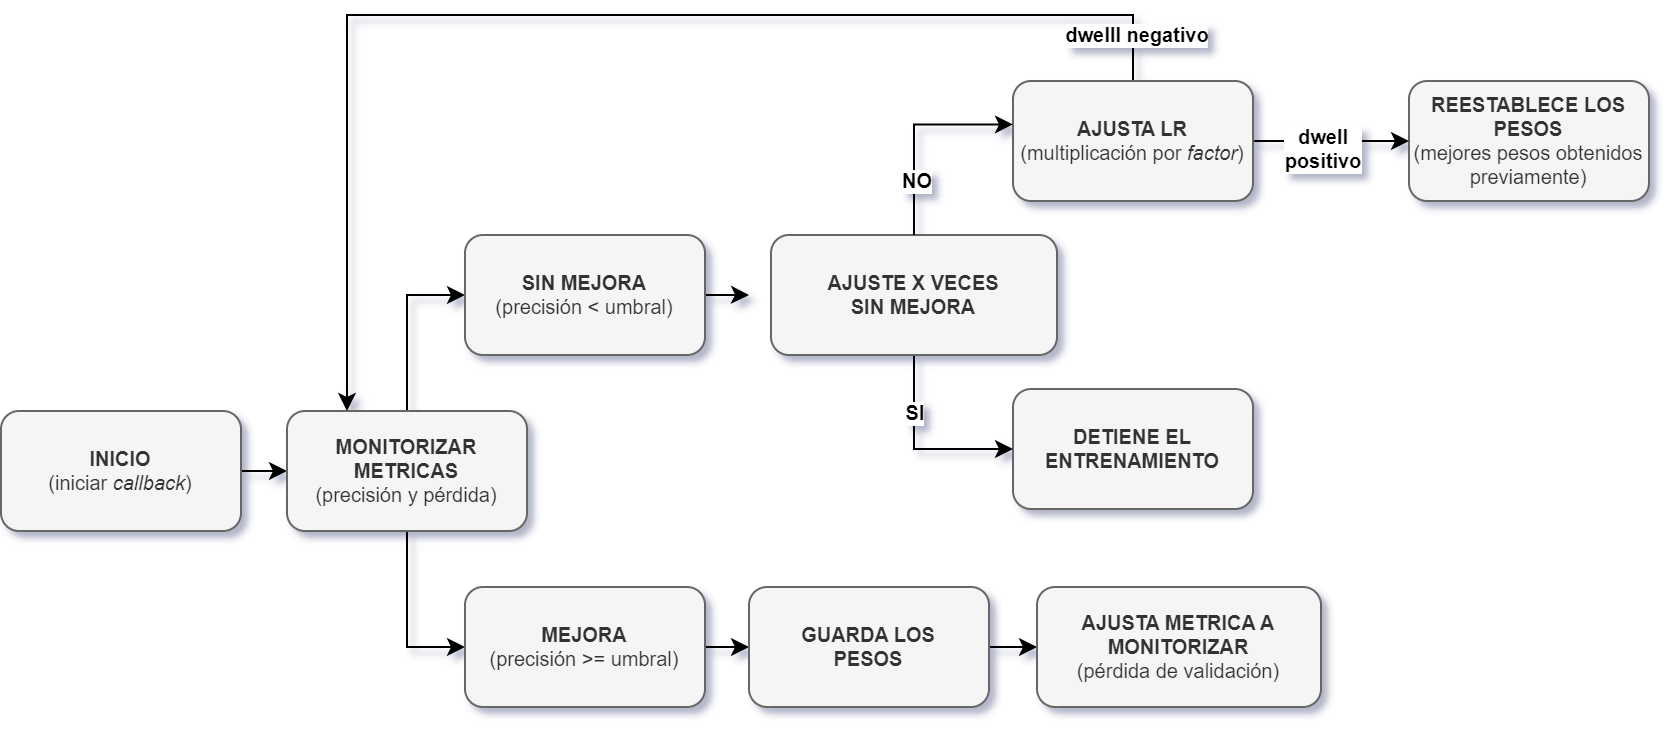
\includegraphics[width=1\textwidth]{./Graphics/lra.drawio.png}
    \caption{Diagrama del algoritmo de ajuste de aprendizaje.}
    \label{fig:lra_permormance}
    \end{center}
  \end{figure}

\textbf{Epochs:} $40$, \textbf{Patience:} 1, \textbf{Stop Patience:} 3, \textbf{Threshold:}  0.9, \textbf{Factor:} 0.5
\end{frame}

\begin{frame}
  \frametitle{Objetivos}

    \begin{block}{Propósitos específicos}
      \small
      \begin{enumerate}
        \item<0> Estudio del estado del arte en diagnóstico de imágenes dermatológicas.
        \item<0> Desarrollo de un modelo de \textit{deep learning} para clasificación.
        \item<0> Mejoras y ajuste de hiperparámetros.
        \item<0-> Optimización de la distribución de datos.
        \item<0-> Implementación de técnicas de validación.
      \end{enumerate}
    \end{block}
\end{frame}


\begin{frame}
  \frametitle{Fuente de Datos: HAM10000}
  \begin{itemize}
    \item Conjunto de datos con 10015 imágenes dermatoscópicas.
    \item Amplia gama de lesiones cutáneas pigmentadas.
  \end{itemize}

  \begin{table}[H]
    \centering
    \small
    \begin{tabular}{lccc}
    \hline
    \textbf{Categoría Diagnóstica} & \textbf{Cantidad} & \textbf{Porcentaje} \\
    \hline
    Melanocytic nevi (NV) & 6705 & 66.95\%  \\
    Melanoma (MEL) & 1113 & 11.11\% \\
    Benign keratosis-like lesions (BKL) & 1099 & 10.97\% \\
    Basal cell carcinoma (BCC) & 514 & 5.13\% \\
    Actinic Keratosis and \\ Intraepithelial Carcinoma (AKIEC) & 327  & 3.27\% \\
    Vascular lesions (VASC) & 142 & 1.42\%  \\
    Dermatofibroma  (DF) & 115 & 1.15\% \\
    \hline
    \end{tabular}
    \caption{Distribución de imágenes por categoría diagnóstica.}
    \label{tab:ham10000_distribution}
 \end{table} 

\end{frame}

\begin{frame}
  \frametitle{Transformación de Datos}

  \begin{itemize}
    \item Transformación de formato \textbf{\textit{one hot encoding}} a formato categórico \textbf{\textit{categorical}}.
  \end{itemize}

  \scalebox{0.5}{
    \begin{tabular}{|c|c|c|c|c|c|c|c|}
      \hline
      \centering
      \textbf{Image} & \textbf{MEL} & \textbf{NV} & \textbf{BCC} & \textbf{AKIEC} & \textbf{BKL} & \textbf{DF} & \textbf{VASC} \\
      \hline
      ISIC\_0024306 & 0 & 1 & 0 & 0 & 0 & 0 & 0 \\
      ISIC\_0024307 & 0 & 1 & 0 & 0 & 0 & 0 & 0 \\
      ISIC\_0024308 & 0 & 1 & 0 & 0 & 0 & 0 & 0 \\
      ISIC\_0024309 & 0 & 1 & 0 & 0 & 0 & 0 & 0 \\
      ISIC\_0024310 & 1 & 0 & 0 & 0 & 0 & 0 & 0 \\
      \hline
    \end{tabular}
  }
  $\rightarrow$
  \scalebox{0.5}{%
    \begin{tabular}{|c|c|}
      \hline
      \textbf{Image} & \textbf{Etiqueta} \\
      \hline
      ISIC\_0024306.jpg & NV \\
      ISIC\_0024307.jpg & NV \\
      ISIC\_0024308.jpg & NV \\
      ISIC\_0024309.jpg & NV \\
      ISIC\_0024310.jpg & MEL \\
      \hline
    \end{tabular}
  }

  \begin{itemize}
    \item <2-> División en entrenamiento, validación y prueba.
    \item <3-> Aumento de datos (\textit{data augmentation}).
    \begin{itemize}
      \item Rango de rotación
      \item Rango de desplazamiento horizontal y vertical
      \item Rango de corte y zoom
      \item Volteo horizontal
      \item Relleno para manejar los píxeles faltantes
    \end{itemize}
  \end{itemize}

\end{frame}


\begin{frame}
  \frametitle{Experimentos Realizados}
  \begin{itemize}
    \item Experimento 1: División asimétrica de datos.
    \item Experimento 2: Estratificación equilibrada de datos.
  \end{itemize}
\end{frame}

\begin{frame}
  \frametitle{Experimentos 1: División asimétrica de datos}

  \begin{itemize}
    \item División en entrenamiento, validación y prueba.
  \end{itemize}

  \begin{table}[H]
   \small
   \centering
   \begin{tabular}{lcc}
   \hline
   \textbf{Categoría diagnóstica} & \textbf{Porcentaje} & \textbf{Cantidad de datos} \\
   \hline
   Entrenamiento & 95\% & $9514$ \\
   Validación    & 2.5\% & $251$  \\
   Prueba        & 2.5\% & $251$  \\ \hline
   \end{tabular}
   
   \label{table:data_distribution_e1}
   \end{table}

  \begin{itemize}
    \item <2-> Establecer la cantidad fija de muestras por clase (300).
    \item <3-> Aplicar \textbf{\textit{class weighting}}.
  \end{itemize}

  \only<3->{
    \begin{table}
      \centering
      \scalebox{0.7}{
        \begin{tabular}{lccc}
          \hline
          Categoría diagnóstica & Muestras  & Pesos\\ \hline
          AKIEC & 300 & 1.00\\
          BCC & 300 & 1.00\\
          BKL & 300 & 1.00\\
          DF & \textcolor{red}{107} & \textcolor{red}{2.60}\\
          MEL & 300 & 1.00\\
          NV & 300 & 1.00\\
          VASC & \textcolor{red}{138} & \textcolor{red}{2.11}\\ \hline
        \end{tabular}
      }
    \end{table}
  }  
\end{frame}

\begin{frame}
  \frametitle{Resultados del experimento 1}

  \begin{figure}[H]
    \begin{center}
        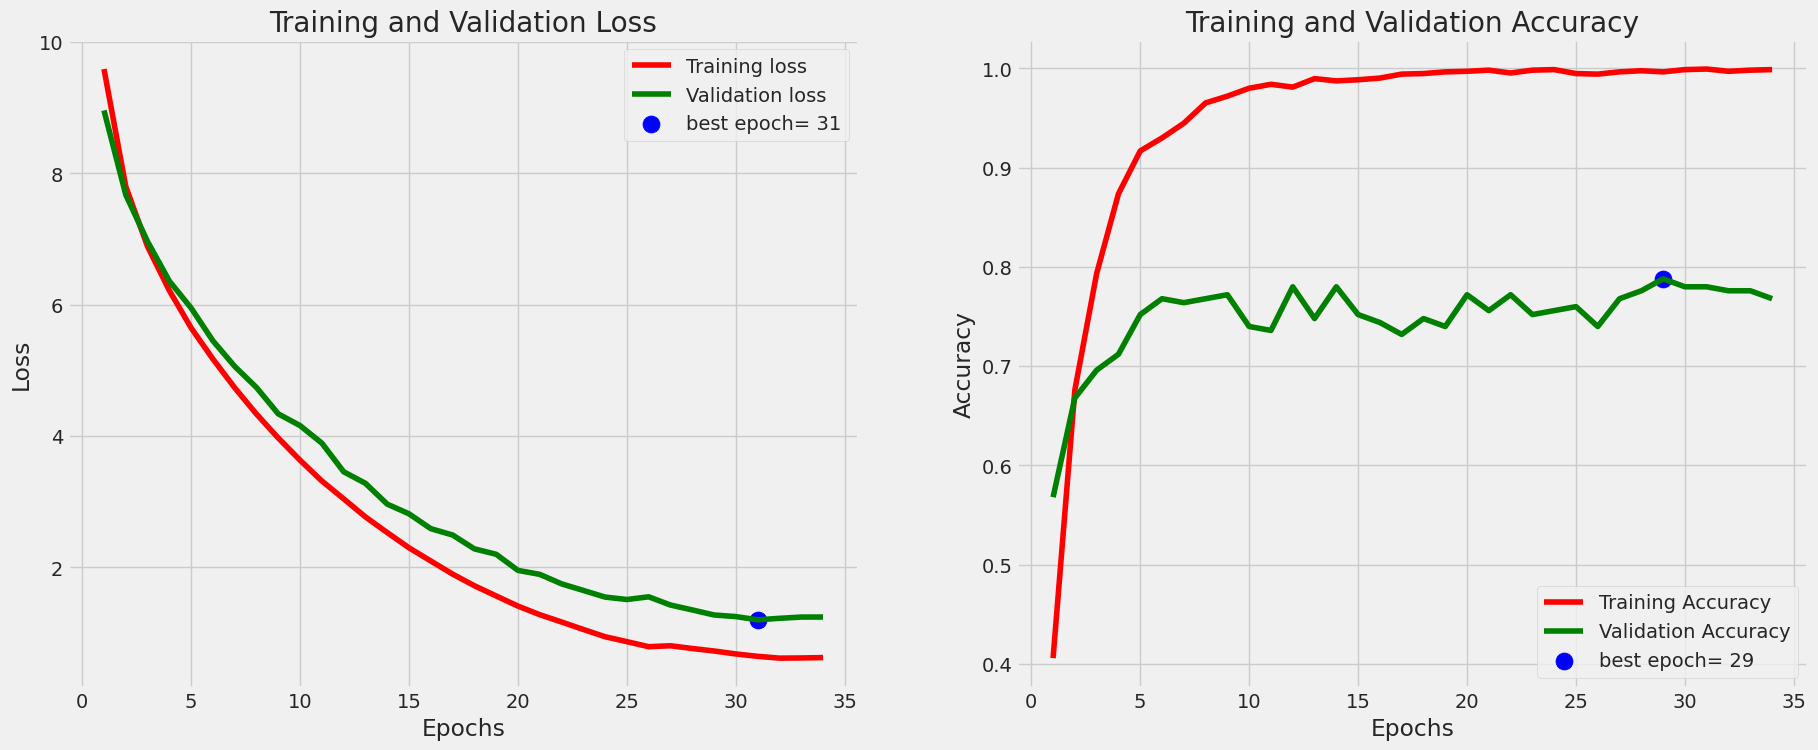
\includegraphics[width=1\textwidth]{./Graphics/training&validation_p1.png}
        \caption{Curva de aprendizaje a lo largo del proceso de entrenamiento del experimento 1.}
    \end{center}
\end{figure}
\end{frame}


\begin{frame}
  \frametitle{Resultados del experimento 1}

  \begin{figure}[H]
    \begin{center}
        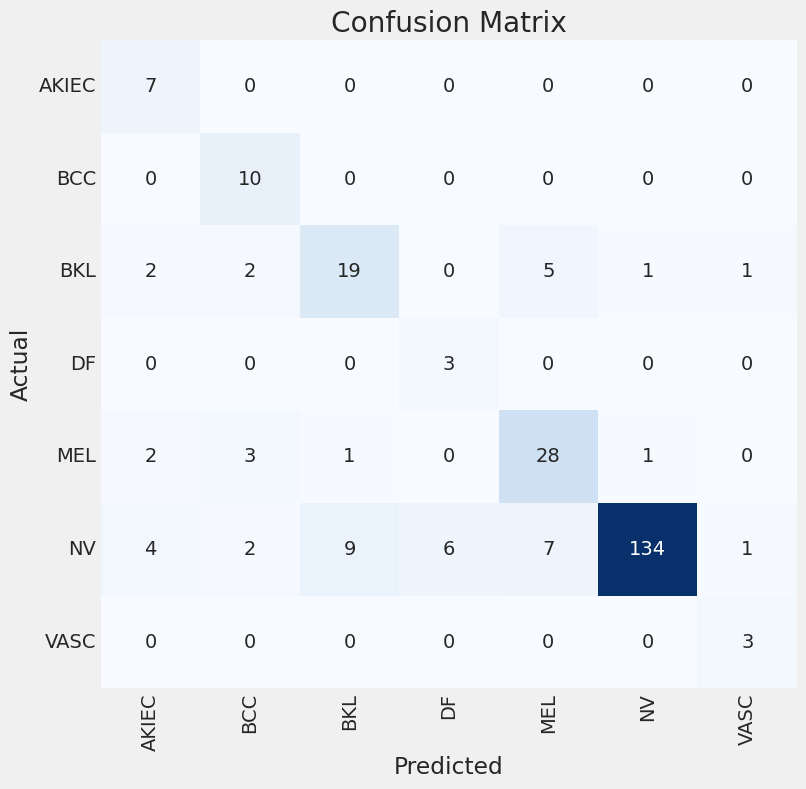
\includegraphics[width=0.7\textwidth]{./Graphics/confussionmatrix_p1.png}
        \caption{Matriz de confusión del experimento 1.}
    \end{center}
  \end{figure}

  % \begin{figure}[H]
  %   \begin{minipage}{0.5\textwidth}
  %     \small
  %       \begin{itemize}
  %         \item \textbf{AKIEC:} 7 correctamente identificadas, 0 errores.
  %         \item \textbf{BCC:} 10 correctamente identificadas, 0 errores.
  %         \item \textbf{BKL:} 19 correctamente identificadas, 2 clasificadas como AKIEC, 2 como BCC, 5 como MEL, 1 como NV, 1 como VASC.
  %       \end{itemize}
  %   \end{minipage}%
  %   \begin{minipage}{0.5\textwidth} 
  %     \small
  %       \begin{itemize}
  %           \item \textbf{DF:} 3 correctamente identificadas.
  %           \item \textbf{MEL:} 28 correctamente identificadas, 2 clasificadas como AKIEC, 3 como BCC,1 como BKL y 1 como NV.
  %           \item \textbf{NV:} 134 correctamente identificadas, errores con varias clases.
  %           \item \textbf{VASC:} 3 correctamente identificadas.
  %       \end{itemize}
  %   \end{minipage}
  % \end{figure}
\end{frame}


% \begin{frame}
%   \frametitle{Resultados del experimento 1}

%   \begin{table}[H]
%     \small
%     \begin{center}
%         \begin{tabular}{|c|c|c|c|c|c|c|c|} \hline
%         E & Loss & Acc & V loss & V acc & LR & M & Batch \\ \hline
%         1 & 9.587 & 40.581 & 8.95658 & 56.800 & $10^{-2}$ & acc & 85.25 \\ \hline
%         2 & 7.798 & 67.615 & 7.67235 & 66.800 & $10^{-2}$ & acc & 21.72 \\ \hline
%         3 & 6.884 & 79.340 & 6.96014 & 69.600 & $10^{-2}$ & acc & 22.56 \\ \hline
%         4 & 6.214 & 87.365 & 6.35865 & 71.200 & $10^{-2}$ & acc & 25.81 \\ \hline
%         5 & 5.646 & 91.690 & 5.94812 & 75.200 & $10^{-2}$ & vloss & 23.08 \\ \hline
%         6 & 5.172 & 92.999 & 5.44954 & 76.800 & $10^{-2}$ & vloss & 23.23 \\ \hline
%         7 & 4.735 & 94.479 & 5.06016 & 76.400 & $10^{-2}$ & vloss & 23.19 \\ \hline
%         8 & 4.334 & 96.528 & 4.73837 & 76.800 & $10^{-2}$ & vloss & 22.90 \\ \hline
%         9 & 3.969 & 97.211 & 4.33689 & 77.200 & $10^{-2}$ & val\_loss & 22.74 \\ \hline
%         10 & 3.631 & 98.008 & 4.15826 & 74.000 & $10^{-2}$ & val\_loss & 22.56 \\ \hline
%         11 & 3.315 & 98.406 & 3.89153 & 73.600 & $10^{-2}$ & val\_loss & 23.11 \\ \hline
%         \dots & \dots & \dots & \dots & \dots & \dots & \dots & \dots \\ \hline
%         34 & 0.627 & 99.886 & 1.24470 & 76.800 & 0.00013 & val\_loss & 23.30 \\ \hline
%         \end{tabular}
%     \end{center}\label{fig:estadisticas_p1}
%   \end{table}
% \end{frame}

\begin{frame}
  \frametitle{Experimentos  2: Estratificación equilibrada de datos}
  
  \begin{itemize}
    \item División en entrenamiento, validación y prueba.
  \end{itemize}

  \begin{table}[H]
    \centering
    \begin{tabular}{lcc}
    \hline
    \textbf{Categoría diagnóstica} & \textbf{Porcentaje} & \textbf{Cantidad de datos} \\
    \hline
    Entrenamiento  & 70\% &  $7010$ \\
    Validación     & 15\% & $1502$  \\
    Prueba         & 15\% & $1503$  \\ \hline
    \end{tabular}
    \label{table:data_distribution_e2}
    \end{table}

  \begin{itemize}
    \item <2-> Establecer la cantidad fija de muestras por clase (500).
  \end{itemize}

  \only<2->{
  \begin{table}[H]
    \centering
    \scalebox{0.7}{
      \begin{tabular}{lccc}
      \hline
      \textbf{Categoría diagnóstica} & \textbf{Entrenamiento} & \textbf{Validación} & \textbf{Prueba} \\
      \hline
      NV    & 500 & 1006 & 1006 \\
      MEL   & 500 & 167  & 167  \\
      BKL   & 500 & 165  & 165  \\
      DF    & 500 & 17   & 17   \\
      AKIEC & 500 & 49   & 49   \\
      BCC   & 500 & 77   & 77   \\
      VASC  & 500 & 21   & 22   \\
      \hline
      \end{tabular}
    }
    \label{tab:train_test_validate_e2}
    \end{table}
  }
\end{frame}


\begin{frame}
  \frametitle{Resultados del experimento 2}

  \begin{figure}[H]
    \begin{center}
        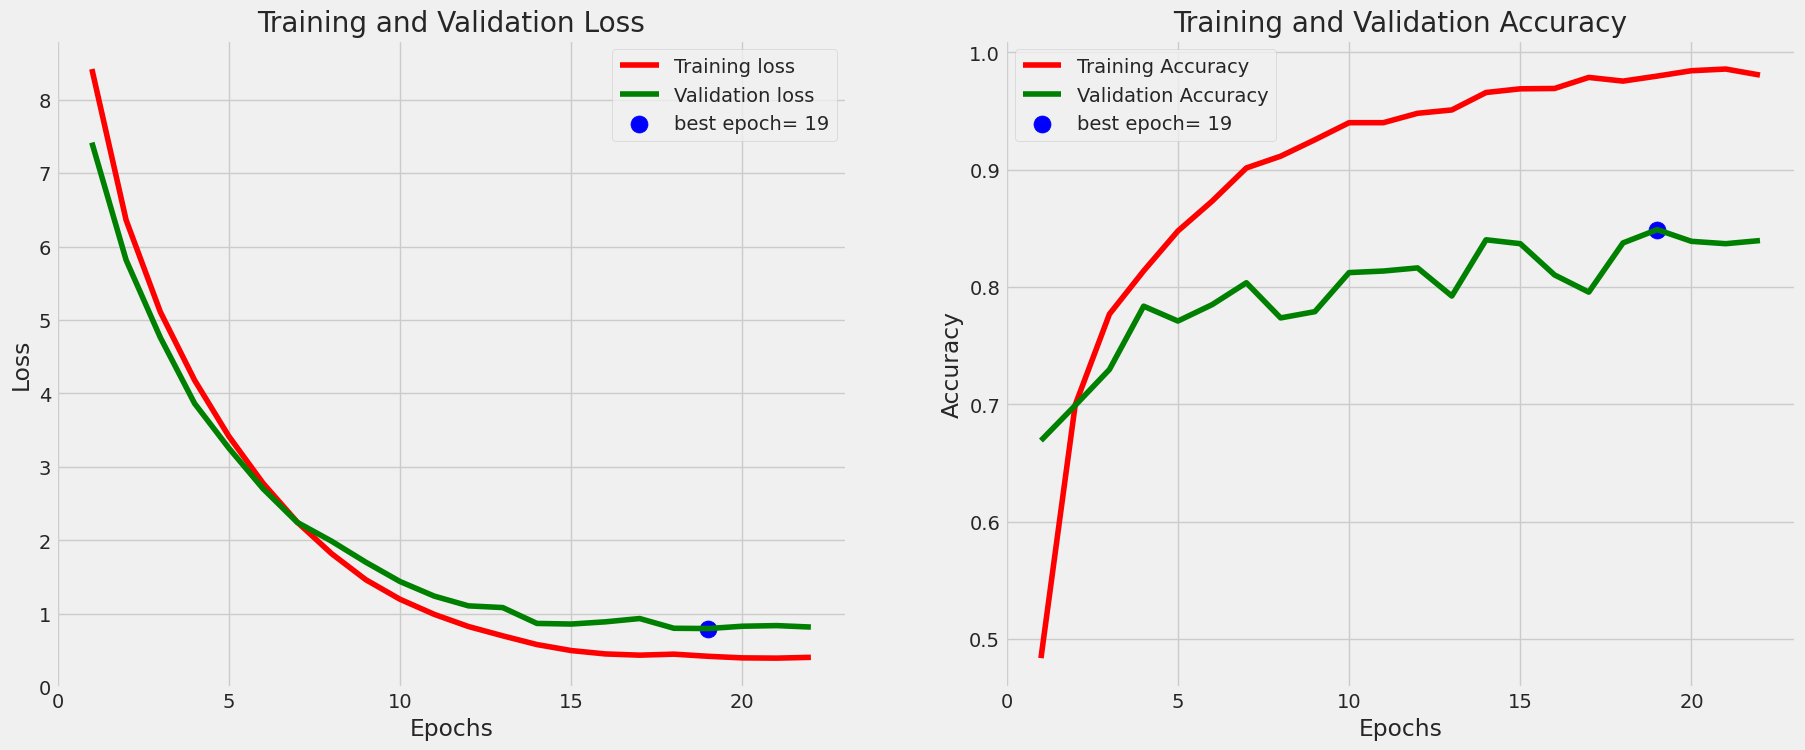
\includegraphics[width=1\textwidth]{./Graphics/training&validation_p3.png}
        \caption{Curva de aprendizaje a lo largo del proceso de entrenamiento del experimento 2.}
    \end{center}
\end{figure}
\end{frame}


\begin{frame}
  \frametitle{Resultados del experimento 2}

  \begin{figure}[H]
    \begin{center}
        \includegraphics[width=0.7\textwidth]{./Graphics/confussionmatrix_p3.png}
        \caption{Matriz de confusión del experimento 2.}
    \end{center}
  \end{figure}

\end{frame}


% \begin{frame}
%   \frametitle{Resultados del experimento 2}

%   \begin{table}[H]
%     \small
%     \begin{center}
%         \begin{tabular}{|c|c|c|c|c|c|c|c|} \hline
%         E & Loss & Acc & V loss & V acc & LR & M & Batch \\ \hline
%         1 & 8.418 & 48.371 & 7.41700 & 66.911 & $10^{-2}$ & accuracy & 184.55 \\ \hline
%         2 & 6.362 & 69.943 & 5.81767 & 69.907 & $10^{-2}$ & accuracy & 107.94 \\ \hline
%         3 & 5.110 & 77.686 & 4.76153 & 72.969 & $10^{-2}$ & accuracy & 106.30 \\ \hline
%         4 & 4.181 & 81.371 & 3.86405 & 78.362 & $10^{-2}$ & accuracy & 104.60 \\ \hline
%         5 & 3.417 & 84.771 & 3.25588 & 77.097 & $10^{-2}$ & accuracy & 101.90 \\ \hline
%         6 & 2.777 & 87.314 & 2.70253 & 78.495 & $10^{-2}$ & accuracy & 101.85 \\ \hline
%         7 & 2.247 & 90.143 & 2.24392 & 80.360 & $10^{-2}$ & val\_loss & 101.98 \\ \hline
%         8 & 1.819 & 91.143 & 1.98878 & 77.364 & $10^{-2}$ & val\_loss & 101.74 \\ \hline
%         9 & 1.464 & 92.543 & 1.70207 & 77.896 & $10^{-2}$ & val\_loss & 101.27 \\ \hline
%         10 & 1.197 & 94.000 & 1.43860 & 81.225 & $10^{-2}$ & val\_loss & 101.71 \\ \hline
%         11 & 0.992 & 94.000 & 1.24007 & 81.358 & $10^{-2}$ & val\_loss & 101.23 \\ \hline
%         \dots & \dots & \dots & \dots & \dots & \dots & \dots & \dots \\ \hline
%         22 & 0.406 & 98.057 & 0.81854 & 83.955 & 0.00006 & val\_loss & 101.18 \\ \hline
%         \end{tabular}
%     \end{center}\label{fig:estadisticas_p2}
% \end{table}
% \end{frame}

\begin{frame}
  \frametitle{Resultados generales}

  \begin{table}
    \footnotesize % Otra opción es \scriptsize
    \setlength{\tabcolsep}{3pt} % Ajusta el espaciado entre columnas
    \centering
    \caption{Informe de clasificación combinado para los experimentos 1 y 2.}
    \label{tab:classification_report_combined}
    \begin{tabular}{lcccccccccc}
    \hline
    & \multicolumn{5}{c}{\textbf{Experimento 1}} & \multicolumn{5}{c}{\textbf{Experimento 2}} \\
    \cline{2-10}
    \textbf{Categoría} & \textbf{Acc} & \textbf{Recall} & \textbf{F1} & \textbf{F2} & \textbf{NM} & \textbf{Acc} & \textbf{Recall} & \textbf{F1} & \textbf{F2} & \textbf{NM} \\
    \hline
    AKIEC & 0.47 & 1.00 & 0.64 & 0.816 & 7   & 0.82 & 0.96 & 0.89 & 0.928  & 49 \\
    BCC   & 0.59 & 1.00 & 0.74 & 0.878 & 10  & 0.81 & 1.00 & 0.90 &  0.955 & 77 \\
    BKL   & 0.66 & 0.63 & 0.64 & 0.636 & 30  & 0.72 & 0.83 & 0.77 & 0.805  & 165 \\
    DF    & 0.33 & 1.00 & 0.50 & 0.711 & 3   & 0.71 & 1.00 & 0.83 & 0.924  & 17 \\
    MEL   & 0.70 & 0.80 & 0.75 & 0.778 & 35  & 0.63 & 0.85 & 0.73 & 0.795  & 167 \\
    NV    & 0.99 & 0.82 & 0.90 & 0.849 & 163 & 0.98 & 0.86 & 0.91 & 0.882  & 1006 \\
    VASC  & 0.60 & 1.00 & 0.75 & 0.882 & 3   & 0.71 & 1.00 & 0.83 & 0.924  & 22 \\
    \hline
    \textbf{Acc} & & & \textcolor{red}{0.81} & & 251 & & & \textcolor{orange}{0.87} & & 1503 \\
    \textbf{MacroAvg} & 0.62 & 0.89 & 0.70 & & 251 & 0.77 & 0.93 & 0.84 & & 1503 \\
    \hline
    \end{tabular}
\end{table}

\end{frame}

% CONCLUSIONES

\begin{frame}
  \frametitle{Conclusiones}
  \begin{itemize}
    \item \textbf{Potencial del aprendizaje profundo:} Alta precisión y eficiencia en diagnóstico de cáncer de piel.
    \item \textbf{Eficacia de la clasificación:} 87\% de eficacia, comparable con los métodos del estado del arte.
    \item \textbf{Comparación entre experimentos:} Mejoras significativas en precisión, recall y puntuaciones F1.
    \item \textbf{Análisis de curvas de aprendizaje:} Convergencia más rápida y mejor generalización en el segundo experimento.
    \item \textbf{Estadísticas de eficacia y matrices de confusión:} Clasificación precisa en varias clases de cáncer de piel.
    \item \textbf{Importancia del conjunto de datos:} Calidad y composición del conjunto de datos HAM10000 como aspectos críticos.
  \end{itemize}
\end{frame}
% RECOMENDACIONES

\begin{frame}
  \frametitle{Recomendaciones: Datos}
  \begin{enumerate}
    \item Enriquecimiento de datos: Añadir más imágenes para robustecer el modelo.
    \item Aumentar la diversidad de datos: Aplicar técnicas de aumento de datos.
    \item Balance de clases mediante aumento: Equilibrar la distribución de clases y distribución representativa en todas las particiones.
  \end{enumerate}
\end{frame}

\begin{frame}
  \frametitle{Recomendaciones: Modelo}
  \begin{enumerate}
    \item Regularización y arquitectura de red: Explorar parámetros de regularización.
    \item Precisión y sesgos: Mejorar clasificación en clases menos representadas.
    \item Optimizadores: Probar con RMSprop o SGD para mejorar rendimiento.
  \end{enumerate}
\end{frame}

% FIN DE LA PRESENTACIÓN

\begin{frame}
  \frametitle{Fin de la presentación}
  \begin{center}
    \Huge{¡Gracias por su atención!}
  \end{center}
\end{frame}

% PREGUNTAS DEL OPONENTE

\begin{frame}
  \frametitle{Preguntas del OPONENTE}

      \begin{enumerate}
        \item<1-> ¿Por qué si EfficientNetB4 tiene mejor precisión se utilizó EfficientNetB1?
        \item<2-> ¿En qué se basaron los parámetros seleccionados de regularización y de la estrategia de cambio de tasa de aprendizaje?
        \item<0> Para las clases con menos elementos (Tabla 3.5 manuscrito) hay clases como la DF que solo tienen 115 elementos, se puede observar según la tabla que estos casos se utilizaron todos los elementos para el entrenamiento y a su vez algunos para validación. Explique en más detalle este proceder  y en caso de ser así, explique brevemente que efecto puede tener esto sobre los resultados de precisión?
        \item<0> Cree que con preprocesamiento más robusto (mejor nitidez, contraste, etc) o con un aumento de parámetros del modelo se puedan mejorar los resultados?
      \end{enumerate}
      
\end{frame}

\begin{frame}
  \frametitle{Pregunta 2}
  \begin{block}{Regularización}
    \begin{itemize}
      \item L2 con $\lambda = 0.016$.
      \begin{itemize}
        \item Valores entre $0.01$ y $0.1$.
        \item Simplicidad del modelo
      \end{itemize} 
      \item L1 con $\lambda = 0.006$.
      \begin{itemize}
        \item Selección de características.
      \end{itemize}
    \end{itemize}
  \end{block}

  \begin{block}{Ajuste de tasa de aprendizaje}
    \begin{itemize}
      \item Se prioriza precisión (\textit{accuracy}) y a partir de un umbral se empieza a priorizar pérdida de validación.
      \item Enfoque de multi-clasificación.
    \end{itemize}
    
  \end{block}
\end{frame}

\begin{frame}
  \frametitle{Preguntas del OPONENTE}

      \begin{enumerate}
        \item<0-> ¿Por qué si EfficientNetB4 tiene mejor precisión se utilizó EfficientNetB1?
        \item<0-> ¿En qué se basaron los parámetros seleccionados de regularización y de la estrategia de cambio de tasa de aprendizaje?
        \item<0-> Para las clases con menos elementos (Tabla 3.5 manuscrito) hay clases como la DF que solo tienen 115 elementos, se puede observar según la tabla que estos casos se utilizaron todos los elementos para el entrenamiento y a su vez algunos para validación. Explique en más detalle este proceder  y en caso de ser así, explique brevemente que efecto puede tener esto sobre los resultados de precisión?
        \item<0> Cree que con preprocesamiento más robusto (mejor nitidez, contraste, etc) o con un aumento de parámetros del modelo se puedan mejorar los resultados?
      \end{enumerate}
\end{frame}

\begin{frame}
  \frametitle{Pregunta 3}

  \begin{table}[H]
    \small
    \centering
    \begin{tabular}{lccc}
    \hline
    \textbf{Categoría diagnóstica} & \textbf{Entrenamiento} & \textbf{Validación} & \textbf{Prueba} \\
    \hline
    NV       & 300 & 158 & 163 \\
    MEL      & 300 & 25  & 35  \\
    BKL      & 300 & 34  & 30  \\
    DF       & \textcolor{green}{107} & 5   & 3   \\
    AKIEC    & 300 & 11  & 7   \\
    BCC      & 300 & 16  & 10  \\
    VASC     & \textcolor{green}{138} & 1   & 3   \\ \hline
    \end{tabular}
    \caption{Distribución de imágenes de cáncer de piel en los conjuntos de entrenamiento, prueba y validación.}
    \label{table:train_test_validate_e1}
    \end{table}
\end{frame}

\begin{frame}
  \frametitle{Preguntas del OPONENTE}

      \begin{enumerate}
        \item<0-> ¿Por qué si EfficientNetB4 tiene mejor precisión se utilizó EfficientNetB1?
        \item<0-> ¿En qué se basaron los parámetros seleccionados de regularización y de la estrategia de cambio de tasa de aprendizaje?
        \item<0-> Para las clases con menos elementos (Tabla 3.5 manuscrito) hay clases como la DF que solo tienen 115 elementos, se puede observar según la tabla que estos casos se utilizaron todos los elementos para el entrenamiento y a su vez algunos para validación. Explique en más detalle este proceder  y en caso de ser así, explique brevemente que efecto puede tener esto sobre los resultados de precisión?
        \item<0-> Cree que con preprocesamiento más robusto (mejor nitidez, contraste, etc) o con un aumento de parámetros del modelo se puedan mejorar los resultados?
      \end{enumerate}
\end{frame}

\begin{frame}
  \frametitle{Fin de la presentación}
  \begin{center}
    \Huge{¡Gracias por su atención!}
    Nuevamente
  \end{center}
\end{frame}

\end{document}
  